\chapter{Implementazione e Architettura del Codice}

Questo capitolo mostra come il modello di dominio e lo schema del database sono stati trasformati in vero codice Java. Il progetto usa un'architettura "a strati" (Layered architecture) basata sul modello BCE, studiata per separare le responsabilità e semplificare la scrittura dei test.

\section{Architettura dei Package}

L'applicazione è organizzata in quattro package principali (Figura \ref{fig:package_diagram}). Le dipendenze tra i package sono rigorosamente direzionali: lo strato di presentazione (\texttt{cli}) non accede mai direttamente al database, ma passa per i \texttt{controllers}, che a loro volta orchestrano il \texttt{domain} e si interfacciano con i \texttt{dao}.

\subsection{cli (Boundary)}
Contiene il punto di ingresso dell'applicazione e la CLI. La classe \texttt{ConsoleMenu} gestisce l'interazione con l'utente, la validazione di input di base e la delega delle operazioni ai Controller.

\subsection{controllers (Control)}
Raccoglie i Controller che implementano i flussi dei casi d'uso. Ogni Controller incapsula la logica di coordinamento, chiama i DAO e applica le regole di business esposte dal Domain Model.

\subsection{domain (Entity)}
Include le entità di dominio (\texttt{Stanza}, \texttt{Prenotazione}, \texttt{Utente} e sottoclassi) e l'implementazione dei Design Pattern principali (State, Strategy, Observer).

\subsection{dao (Persistence)}
Contiene le interfacce DAO, le implementazioni PostgreSQL e l'oggetto \texttt{ConnectionManager}. L'obiettivo è isolare la persistenza e mantenere il dominio indipendente dalla tecnologia di storage.

\section{Livello di Persistenza (Pattern DAO)}

Per non mischiare la logica dell'applicazione con il codice SQL, l'accesso a PostgreSQL è gestito dal pattern \textbf{Data Access Object (DAO)}. In questo modo la business logic non sa (e non deve sapere) nulla di come funziona materialmente il database.

La connessione al database è gestita tramite un \textbf{Singleton Pattern} (\texttt{ConnectionManager}), che assicura l'esistenza di un'unica istanza di connessione (o di un connection pool) condivisa per tutta l'applicazione, evitando l'overhead di connessioni multiple.

\begin{lstlisting}[caption={Interfaccia generica DAO (\texttt{GenericDAO.java})}, label={lst:dao_interface}]
public interface GenericDAO<T, ID> {
    void save(T entity);
    T findById(ID id);
    List<T> findAll();
    void update(T entity);
    void delete(ID id);
}
\end{lstlisting}

\begin{lstlisting}[caption={Specializzazione per il dominio (\texttt{StanzaDAO.java})}, label={lst:stanza_dao}]
public interface StanzaDAO extends GenericDAO<Stanza, String> {
    List<Stanza> findBySedeAndStato(String sedeId, String statoCorrente);
}
\end{lstlisting}

In modo analogo, \texttt{PrenotazioneDAO} e \texttt{WaitingListDAO} incapsulano le operazioni di persistenza per prenotazioni e liste d'attesa.

\section{Configurazione della Connessione al Database}
Le credenziali di accesso al database non sono hardcoded: vengono lette da \texttt{db.properties} (in \texttt{src/main/resources}) o da variabili d'ambiente, separando configurazione e codice ed evitando la pubblicazione accidentale di segreti.

\begin{lstlisting}[caption={Caricamento della configurazione DB dal classpath}]
Properties props = loadProperties();
String url = firstNonBlank(
    System.getenv("EM_DB_URL"),
    System.getProperty("db.url"),
    props.getProperty("db.url"),
    "jdbc:postgresql://localhost:5432/escapemanager"
);
\end{lstlisting}

\section{Validazione Input e Gestione Errori}
La CLI valida i formati di input (numeri, date e orari) prima di invocare i Controller. Le eccezioni di business (\texttt{ValidationException} e sottoclassi) propagano errori gestibili dalla UI, mantenendo la logica di validazione separata dalla presentazione.

\section{Implementazione dei Design Pattern}

Di seguito vengono riportati i frammenti di codice più significativi che mostrano l'implementazione pratica dei Design Pattern progettati nel Capitolo 3.

\subsection{State Pattern}
Lo State Pattern elimina la necessità di costrutti condizionali complessi per la gestione del ciclo di vita della \texttt{Stanza}. Ogni stato concreto implementa il comportamento specifico e gestisce, ove necessario, la transizione allo stato successivo.

\begin{lstlisting}[caption={Interfaccia dello State Pattern (\texttt{RoomState.java})}, label={lst:state_interface}]
public interface RoomState {
    void prenota(Stanza stanza);
    void iniziaSessione(Stanza stanza);
    void terminaSessione(Stanza stanza);
    void setManutenzione(Stanza stanza);
    void setDisponibile(Stanza stanza);
    String getStatusString();
}
\end{lstlisting}

\begin{lstlisting}[caption={Stato concreto (\texttt{DisponibileState.java})}, label={lst:state_concrete}]
public class DisponibileState implements RoomState {
    @Override
    public void iniziaSessione(Stanza stanza) {
        stanza.setStato(new InCorsoState()); // Transizione di stato
    }
    
    @Override
    public void terminaSessione(Stanza stanza) {
        throw new IllegalStateException(
            "Impossibile terminare una sessione per una stanza DISPONIBILE.");
    }
    // ... altri metodi
}
\end{lstlisting}

\begin{approfondimento}
\textbf{State Pattern vs Strategy Pattern}

Lo \textbf{State Pattern} e lo \textbf{Strategy Pattern} condividono la stessa struttura meccanica: entrambi delegano il comportamento a un oggetto che implementa un'interfaccia comune, favorendo il polimorfismo rispetto ai costrutti condizionali. Tuttavia, differiscono nell'\textit{intento}:
\begin{itemize}
    \item \textbf{Strategy}: l'algoritmo viene scelto \textit{una tantum} dall'esterno (es. l'Admin seleziona \texttt{TariffaWeekend}) e resta fisso per la durata dell'operazione. Le strategie sono intercambiabili ma non si sostituiscono autonomamente.
    \item \textbf{State}: l'oggetto \textit{transiziona automaticamente} tra stati in base alla propria logica interna. Ad esempio, \texttt{DisponibileState} sa che dopo \texttt{iniziaSessione()} lo stato diventa \texttt{InCorsoState}. La transizione è governata dallo stato stesso, non dal client.
\end{itemize}
Nel progetto, questa distinzione è evidente: la \texttt{PricingStrategy} viene impostata esplicitamente dal \texttt{TariffeController}. Al contrario, il \texttt{RoomState} si auto-sostituisce: ogni stato concreto invoca \texttt{stanza.setStato()} all'interno dei propri metodi di transizione, senza intervento esterno.
\end{approfondimento}

\subsection{Strategy Pattern}
Il calcolo del prezzo della prenotazione (UC1) è demandato alla \texttt{PricingStrategy}. L'Admin, tramite il \texttt{TariffeController}, seleziona la strategia appropriata e la imposta sulla stanza.

\begin{lstlisting}[caption={Interfaccia dello Strategy Pattern (\texttt{PricingStrategy.java})}, label={lst:strategy_interface}]
public interface PricingStrategy {
    double calcola(double prezzoBase, int numeroGiocatori);
}
\end{lstlisting}

\begin{lstlisting}[caption={Strategia concreta (\texttt{TariffaWeekend.java})}, label={lst:strategy_concrete}]
public class TariffaWeekend implements PricingStrategy {
    private static final double SOVRAPPREZZO = 1.20; // +20%
    
    @Override
    public double calcola(double prezzoBase, int numeroGiocatori) {
        return (prezzoBase * numeroGiocatori) * SOVRAPPREZZO;
    }
}
\end{lstlisting}

\subsection{Observer Pattern}
La lista d'attesa (UC2) implementa un sistema Publisher-Subscriber puro in Java, disaccoppiando l'evento di cancellazione di una prenotazione dall'invio effettivo delle notifiche.

\begin{lstlisting}[caption={Interfaccia Observer (\texttt{WaitingListObserver.java})}, label={lst:observer_interface}]
public interface WaitingListObserver {
    void update(Stanza stanza, LocalDateTime slotLiberato);
}
\end{lstlisting}

\begin{lstlisting}[caption={Subject concreto (\texttt{WaitingList.java})}, label={lst:observer_subject}]
public class WaitingList {
    private List<WaitingListObserver> observers = new ArrayList<>();

    public void attach(WaitingListObserver observer) {
        observers.add(observer);
    }

    public void notifyObservers(Stanza stanza, LocalDateTime slot) {
        for (WaitingListObserver obs : observers) {
            obs.update(stanza, slot);
        }
    }
}
\end{lstlisting}

\subsection{Builder Pattern}
La classe \texttt{Prenotazione} richiede 7 parametri diversi nel costruttore. Per evitare confusione con l'ordine delle variabili ho usato il pattern creazionale \textbf{Builder}, che rende il codice molto più leggibile quando si devono inizializzare molti attributi.

\begin{lstlisting}[caption={Builder Pattern per la classe Prenotazione}, label={lst:builder_pattern}]
Prenotazione p = new Prenotazione.Builder()
        .id(UUID.randomUUID().toString())
        .clienteId("C01")
        .stanzaId("R01")
        .dataOra(LocalDateTime.of(2026, 10, 31, 21, 0))
        .numeroGiocatori(4)
        .prezzoTotale(80.0)
        .statoPartita("CONFERMATA")
        .build();
\end{lstlisting}

\section{Dependency Injection e Testabilità}
I Controller ricevono i DAO tramite costruttore, facilitando la sostituzione delle dipendenze in fase di test. La CLI si limita a comporre l'oggetto e a delegare, mantenendo separati input/output e logica di business.

\begin{lstlisting}[language=Java, caption=Iniezione delle dipendenze nel controller]
PrenotazioneDAO prenotazioneDAO = factory.getPrenotazioneDAO();
StanzaDAO stanzaDAO = factory.getStanzaDAO();
PrenotazioneController controller = new PrenotazioneController(prenotazioneDAO, stanzaDAO);
\end{lstlisting}

\section{Gestione Centralizzata delle Eccezioni (Information Hiding)}
Per il controllo degli errori ho evitato le eccezioni base di Java (come \texttt{RuntimeException}), preferendo una gerarchia di eccezioni custom derivata da \texttt{EscapeManagerException}.

Come illustrato nella Figura \ref{fig:class_diagram_persistence}, la gerarchia divide formalmente gli errori in base al layer architetturale in cui si verificano:
\begin{itemize}
    \item \textbf{\texttt{ValidationException}:} utilizzata dal dominio per segnalare violazioni delle invarianti di business (es. la sottoclasse \texttt{SlotNonDisponibileException}).
    \item \textbf{\texttt{DatabaseException}:} utilizzata dal layer DAO per incapsulare problemi di persistenza.
\end{itemize}

\begin{figure}[H]
    \centering
    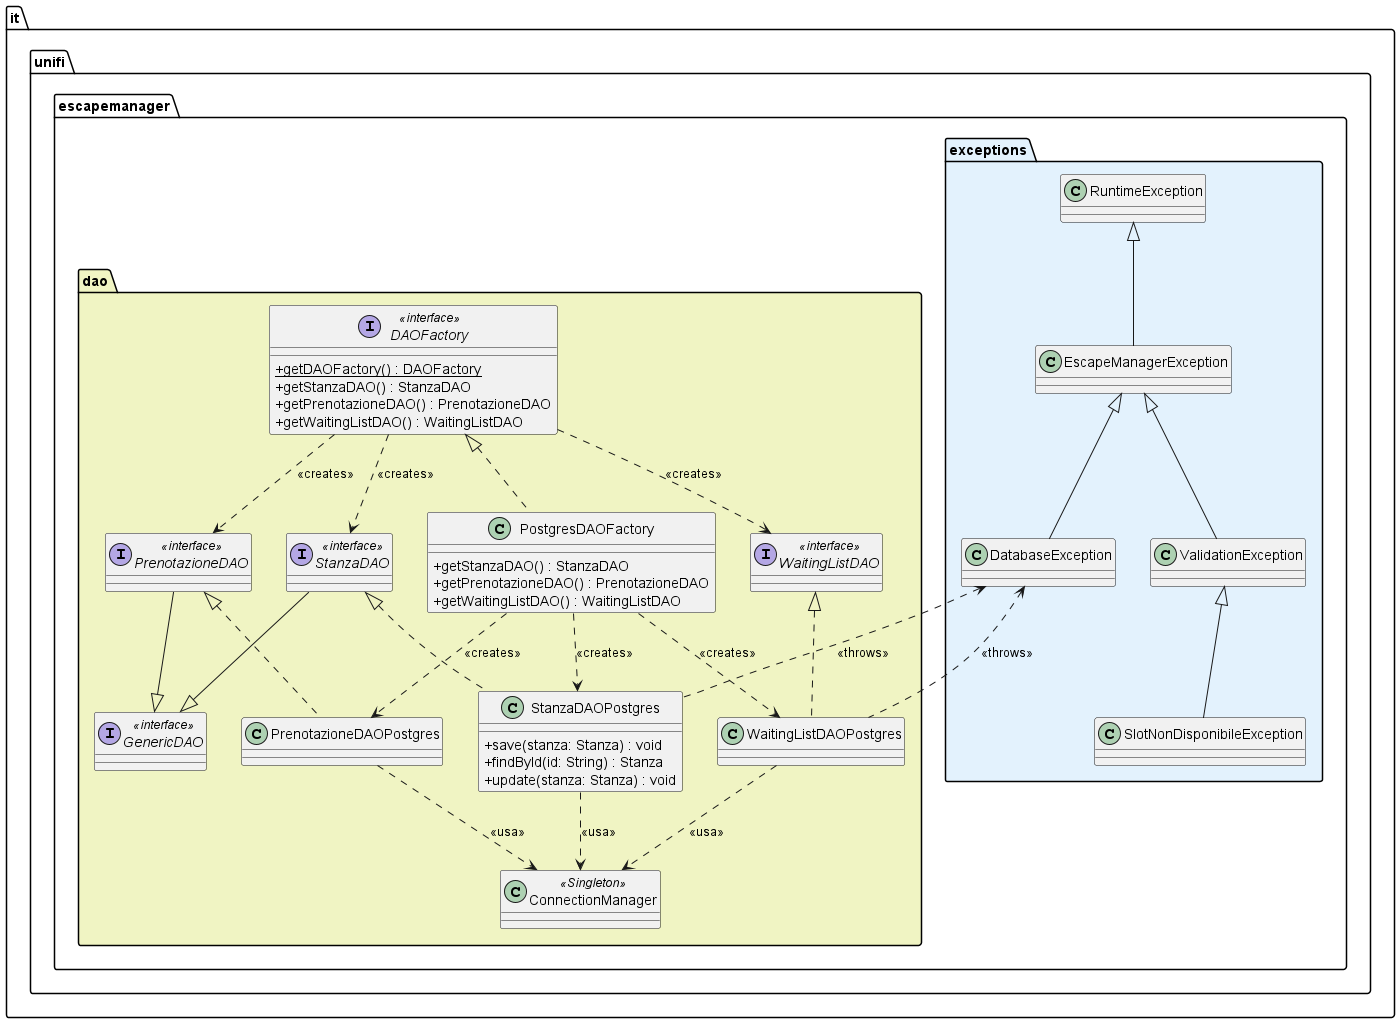
\includegraphics[width=0.85\textwidth]{images/class_diagram_persistence.png}
    \caption{Diagramma delle Classi: Pattern DAO Factory e Gerarchia Eccezioni}
    \label{fig:class_diagram_persistence}
\end{figure}

Questo approccio maschera i dettagli tecnici (Information Hiding): se il driver JDBC lancia una \texttt{SQLException}, il livello DAO la cattura e la trasforma in una \texttt{DatabaseException}. Così facendo, il Controller che riceve l'errore non deve preoccuparsi di questioni legate a SQL o al driver.

\begin{lstlisting}[language=Java, caption=Incapsulamento delle eccezioni SQL nel layer DAO]
try (PreparedStatement stmt = conn.prepareStatement(query)) {
    // Esecuzione query...
} catch (SQLException e) {
    // La SQLException originaria viene nascosta ai livelli superiori
    throw new DatabaseException("Errore di accesso ai dati durante il salvataggio.", e);
}
\end{lstlisting}

\section{Gerarchia delle Interfacce e Liskov Substitution Principle}
Ho creato l'interfaccia \texttt{GenericDAO<T, ID>} per avere un contratto di base CRUD per tutte le entità. Le sotto-interfacce come \texttt{StanzaDAO} aggiungono le interrogazioni specifiche, e le classi concrete come \texttt{StanzaDAOPostgres} contengono le vere query SQL. 

Questo design rispetta il \textbf{Liskov Substitution Principle (LSP)}: il blocco dei \textit{Controller} comunica solo con l'astrazione (\texttt{StanzaDAO}) e ignora totalmente quale sia la classe concreta fornita in quel momento.

\begin{lstlisting}[language=Java, caption=Gerarchia delle interfacce DAO]
public interface GenericDAO<T, ID> {
    void save(T entity);
    T findById(ID id);
    List<T> findAll();
    void update(T entity);
    void delete(ID id);
}

// Specializzazione per il dominio: aggiunge query domain-specific
public interface StanzaDAO extends GenericDAO<Stanza, String> {
    List<Stanza> findBySedeAndStato(String sedeId, String statoCorrente);
}
\end{lstlisting}

\section{Copia Difensiva (Defensive Copy)}
Per tenere al sicuro i dati ho usato una tecnica chiamata \textbf{copia difensiva}. La classe \texttt{WaitingList} contiene internamente la lista degli iscritti (Observer). Se fornissi la lista tramite un classico getter, chiunque potrebbe manipolarla dall'esterno. Per proteggerla (Information Hiding), \texttt{getObservers()} ne restituisce una versione in sola lettura:

\begin{lstlisting}[language=Java, caption=Copia difensiva nella WaitingList]
public List<WaitingListObserver> getObservers() {
    return Collections.unmodifiableList(observers);
}
\end{lstlisting}

Qualsiasi tentativo di aggiungere o rimuovere elementi dalla lista restituita causerà una \texttt{UnsupportedOperationException}, proteggendo l'integrità dell'incapsulamento.



